\subsection{Ergebnisse}
\label{sec:study_results_quantitativ}

\subsubsection{Übersicht}

\begin{longtable}{|l|l|c|}
    \hline
                        &           & \textbf{Anzahl} \\ \hline
    Teilnehmer          & insgesamt & 9 745 \\
                        & gefiltert & 4 012 \\ \hline
    Gefahrene Routen    & insgesamt & 41 540 \\
                        & gefiltert & 16 531 \\ \hline
\caption{}
\label{tab:study_user_overview}
\end{longtable}

Um bei der Analyse der Daten, Nutzer auszuschließen, die eine Navigation nur gestartet haben, um sich diese anzusehen, aber NUNAV nicht aktiv während einer Autofahrt genutzt haben werden Routen, die kürzer als 5 Kilometer sind herausgefiltert. 
%Dies verhindert außerdem, dass das Gelangen zur ersten Route, sowie das Suchen von Parkplätzen einen zu großen Einfluss auf die Daten haben

Für Nutzer der Gruppen 3 und 4 kann es passieren, dass sie keine Erklärung während der Navigation erhalten, wenn die aktuelle Route keiner Erklärung bedarf. Dies ist der Fall, wenn das Verkehrsaufkommen \glqq normal\grqq{} ist und der Nutzer während der gesamten Fahrt guten GPS-Empfang hat (Definitionen siehe \autoref{sec:gps_accuracy_definition}). Bei der Betrachtung von einzelnen Routen werden die Teilnehmer folglich in die Gruppen 1 oder 2 umsortiert, falls sie während der Navigation keine Erklärung gesehen haben. Wird eine Metrik analysiert, die sich pro Nutzer über mehrere Routen erstreckt, werden die Teilnehmer den Gruppen zugeordnet, wenn NUNAV ihnen mindestens einmal eine Erklärung aus der Studiengruppe angezeigt hat. Über Übersicht findet sich in \autoref{tab:study_user_group_overview}

\begin{table}
    \begin{center}
        \begin{tabular}{|l|c|c|c|}
            \hline
            \multirow{2}{*}{\textbf{Gruppe}} & \multirow{2}{*}{\textbf{Anzahl der Nutzer}} & \multicolumn{2}{|c|}{\textbf{Anzahl der Routen}} \\ \cline{3-4}
            & & Insgesamt & Mit Nutzerbewertung \\ \hline \hline
            Gruppe 1            & 1 778  & 4 807  & 133 \\ \hline
            Gruppe 2            & 1 397  & 3 413  & 135 \\ \hline
            Gruppe 3            & 468   & 4 571  & 184 \\ \hline
            Gruppe 4            & 369   & 3 740  & 173 \\ \hline \hline
            \textbf{Insgesamt}  & 4 012  & 16 531 & 625 \\ \hline
        \end{tabular}
    \end{center}
    \caption{Übersicht über die Daten der Studiengruppen}
    \label{tab:study_user_group_overview}
\end{table}

\subsubsection{Einflüsse außerhalb von Erklärungen}

Um auszuschließen, dass die untersuchten Variablen von weiteren Faktoren abhängen habe wurde zu Beginn geprüft, ob eine schlecht vorausgesagte Ankunftszeit oder mehrfach auftretendes schlechtes GPS einen Effekt auf die Anzahl der Abweichungen von der Route oder die Zufriedenheit mit der Route haben. Dies geschieht, da es Vermutungen eines negativen Zusammenhangs gab, der die Ergebnisse der Untersuchung der integrierten Erklärungen beeinflussen könnte. Dazu wurde die Kontrollgruppe (Gruppe 1: Ohne Erklärungen) untersucht.

Die 4 Hypothesen lauten wie folgt:

\begin{enumerate}
    \item[1.1] WENN die ATA mehr als 10 \% und mindestens 2 Minuten von der ETA abweicht, DANN hat dies einen signifikant messbaren negativen Einfluss auf die Nutzerzufriedenheit.
    \item[1.2] WENN die ATA mehr als 10 \% und mindestens 2 Minuten von der ETA abweicht, DANN ist die Anzahl der Routenabweichungen signifikant messbar höher.
    \item[1.3] WENN NUNAV auf der betrachteten Route pro 5 km durchschnittlich mindestens eine Positionsungenauigkeit aufwies, DANN hat dies einen signifikant messbaren negativen Einfluss auf die Nutzerzufriedenheit.
    \item[1.4] WENN NUNAV auf der betrachteten Route pro 5 km durchschnittlich mindestens eine Positionsungenauigkeit aufwies, DANN ist die Anzahl der Routen-Abweichungen signifikant messbar höher.
\end{enumerate}

Bei der statistischen Prüfung der Auswirkung von schlecht vorausgesagte Ankunftszeit auf die Anzahl der Routen-Abweichungen mittels eines Kruskal-Wallis-Tests lässt sich kein Haupteffekt feststellen ($ p = 0.197648 > 0.05 $). Gleiches gilt für die Überprüfung eines Effektes auf die Nutzerzufriedenheit ($ p = 0.564911 > 0.05 $). Folglich können die Hypothesen 1.1 und 1.2 abgelehnt werden.

Für die Überprüfung, ob eine schlechte Positionierung einen Effekt auf die Nutzerzufriedenheit hat, hat ein Kruskal-Wallis-Test ergeben, dass kein signifikanter Effekt vorliegt ($ p = 0.269231 > 0.05 $). Folglich kann Hypothese 1.3 abgelehnt werden. Bei der Prüfung von Hypothese 1.4 hat sich herausgestellt, dass die Anzahl der Routen-Abweichungen signifikant höher ist, wenn es im Durchschnitt mehr als ein mal pro 5 km eine Positionsungenauigkeit gibt ($ p = 3.426601e-15 < 0.05 $  $ \mu_{good gps}=efse $ $ \mu_{bad gps}=efse $). Folglich kann Hypothese 1.4 angenommen werden. Da eine häufige ungenaue Positionierung also bereits einen Einfluss auf die Anzahl der Abweichungen von der Route hat, werden Daten mit ungenauer Positionierung bei der Auswertung vom Einfluss von Erklärungen auf die Anzahl der Routen-Abweichungen nicht mitbetrachtet.

\subsubsection{Nutzerabweichungen von der vorgeschlagenen Route}

\textbf{Hypothesen}

\begin{enumerate}
    \item[2.1] WENN der Teilnehmer Erklärungen erhält, DANN folgt er signifikant häufiger der vorgeschlagenen Route als wenn er keine erhält.
    \item[2.2] WENN der Teilnehmer nur eine der beiden vorgestellten Erklärungstypen erhält, DANN folgt er signifikant weniger häufig der vorgeschlagenen Route als wenn ihm beide Arten von Erklärungen präsentiert werden.
\end{enumerate}

 Als Messwert wird die Anzahl der \textit{Offroutes} relativ zu Gesamtlänge der Route verwendet. Die Einheit ist Offroute pro Kilometer.

\smallskip

\noindent\colorbox{lightgray}{%
    \parbox{0.975\linewidth}{
        \textbf{Definition}

        Ein \textit{Offroute} ist der Fall, dass der Nutzer sich aktuell nicht auf der vorgeschlagenen Route befindet. Konkret bedeutet dies, dass das Smartphone NUNAV eine neue Position bereitstellt und nach einer Evaluation bestimmter Kriterien festgestellt wird, dass sich der Nutzer nicht mehr auf der Route befindet. In der Regel wird dann eine neue Route vom Server angefordert.
        
        \textit{Zu Beachten}
        \begin{itemize}
            \item Bis der Nutzer eine neue Route erhält, kann es mehrere \textit{Offroutes} geben.
            \item Es kann sein, dass der Nutzer mehrfach wieder die gleiche Route nach einem \textit{Offroute} erhält.
            \item Es kann auch zu einem \textit{Offroute} kommen, wenn die Nutzerposition schlecht ist.
        \end{itemize}
    }
}

\smallskip

Bei der Betrachtung von Abweichungen von der Route werden wie oben beschrieben Navigationen, bei denen es häufig zu einer ungenauen Positionierung kommt aus den Daten gefiltert. Außerdem wurde sie normalisiert, sodass schlussendlich 16 314 einzelne Navigationen zur Analyse der Routen-Abweichungen im Datensatz verblieben sind.

\begin{figure}
    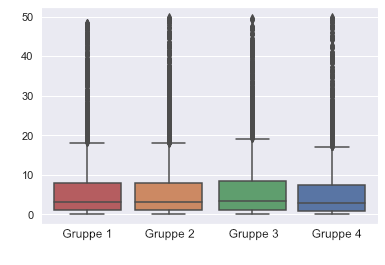
\includegraphics[width=0.8\textwidth]{contents/06_model_evaluation/res/OffRoute_Result_Overview.png}
    \caption{Anzahl der Offroutes pro Kilometer für jede Studiengruppe}
\end{figure}

\begin{table}
    \begin{center}
        \begin{tabular}{|l|c|c|}
            \hline
            \textbf{Studiengruppe}  & \textbf{Mittelwert} [N/km] & \textbf{Standardabweichung} [N/km]\\ \hline
            Gruppe 1                & 0.0753 & 0.1293 \\ \hline
            Gruppe 2                & 0.0786 & 0.1272 \\ \hline
            Gruppe 3                & 0.0803 & 0.1410 \\ \hline
            Gruppe 4                & 0.0732 &  0.1328 \\ \hline
        \end{tabular}
    \end{center}
    \caption{Übersicht der Ergebnisse der Routen-Abweichungen pro Kilometer}
    \label{tab:study_offroute_results}
\end{table}

Um zu prüfen, ob die Unterschiede der Mittelwerte signifikant sind, muss dies mittels eines statistischen Tests überprüft werden. Da es sich um ein Experiment von meheeren nicht zusammenhängenden Studiengruppen mit mehr als zwei verschiedenen Bedingungen handelt, kommen entweder ein ANOVA- oder Kruskal-Wallis-Test infrage. Für ersteren gilt, dass die Daten gleich verteilt sein müssen. Dies wurde mittels Shapiro-Wilk-Test geprüft. Da das Ergebnis für alle Test-Gruppen $ p = 0.0 < 0.05 $ ist, sind die Daten nicht normal verteilt. Folglich wird zur Signifikanzprüfung der Kruskal-Wallis-Test verwendet. Aufgrund des Ergebnisses von $ p = 0.000007 < 0.05 $, wird abgeleitet, dass ein Haupteffekt vorliegt.

Für die Prüfung zwischen welchen Studiengruppen ein signifikanter Unterschied vorliegt, wird der Dunn-Test \cite{dunn1964multiple} verwendet. (P wird mit der \glqq bonferoni\grqq{}-Methode korrigiert.)

Auch hier wird wieder von einem Signifikanzniveau $ p < 0.05 $ ausgegangen (Siehe \autoref{sec:appendix_study_results}). Folglich weichen die Nutzer der Gruppe 4 signifikant weniger von der vorgeschlagenen Route ab als die Teilnehmer aller anderen Gruppen ($ p_{11} = 0.0288 $, $ p_{12} = 0.0000 $, $ p_{13} = 0.0030 $). Weitere signifikante Unterschiede gibt es nicht.

Hypothese 2.1 trifft zwar für das Geben aller Erklärungstypen (Gruppe 4) zu, nicht aber für die Gruppen 2 und 3. Folglich wird diese abgelehnt. Hypothese 2.2 kann angenommen werden, da die Nutzer der Gruppe 4 sowohl signifikant weniger von der vorgeschlagenen Route abgewichen sind als die Nutzer der Gruppe 2 sind als auch die Nutzer der Gruppe 3.

\subsubsection{Nutzerzufriedenheit mit der aktuellen Route}

Um die Zufriedenheit der Nutzer mit der abgeschlossenen Navigation zu evaluieren, setzt NUNAV auf eine Bewertung mithilfe von 5 Sternen bei Erreichen des Zieles. Dies ist verknüpft mit der Frage \glqq Wie hat dir die Fahrt gefallen\grqq (Siehe \autoref{fig:screenshot_destination_reached}). Außerdem sind die Fahrtdauer und zurückgelegte Kilometer angegeben.

\begin{figure}
    
\includegraphics[width=0.25\linewidth]{contents/res/missing_image.pdf}
    \caption{Bildschirmfoto der Bewertungsdialogs}
    \label{fig:screenshot_destination_reached}
\end{figure}

\textbf{Hypothesen}

\begin{enumerate}
    \item[3.1] WENN Teilnehmer Erklärungen erhalten, DANN geben sie im Vergleich eine signifikant höhere Bewertung für die Navigation ab, als wenn sie keine Erklärungen erhalten.
    \item[3.2] WENN Teilnehmer nur einen der beiden vorgestellten Erklärungstypen erhalten, DANN geben sie im Vergleich eine signifikant niedrigere Bewertung für die Navigation ab, als wenn sie beide Erklärungstypen erhalten.
\end{enumerate}

\begin{figure}
    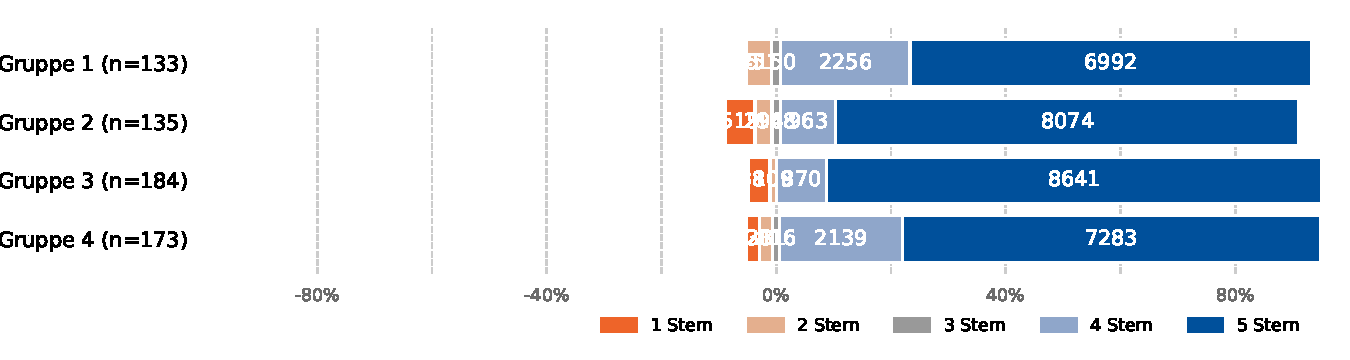
\includegraphics[width=\linewidth]{contents/06_model_evaluation/res/Rating_Result_Overview.pdf}
    \caption{Verteilung der Teilnehmer-Bewertung der Navigation für jede Studiengruppe bezogen auf die insgesamt abgegebenen Bewertungen}
    \label{fig:Rating_Result_Overview}
\end{figure}

Für die Prüfung zwischen welchen Studiengruppen ein signifikanter Unterschied vorliegt, wird wieder der Dunn-Test \cite{dunn1964multiple} verwendet, nachdem ein Kruskal-Wallis-Test einen Haupteffekt zeigt ($ p = 0.00335 $). Daraus resultiert, dass es zwischen den Gruppen 1 und 3 ($ p = 0.005723$) sowie 3 und 4 ($ p = 0.024375 $) einen signifikanten Unterschied bei der Zufriedenheit mit der aktuellen Route gibt. Mithilfe von \autoref{fig:Rating_Result_Overview} wird abgeleitet, dass es insbesondere mehr 5-Stern-Bewertungen in Gruppe 3 gegenüber den Gruppen 1 und 4 gibt. Die Anteile der ein und zwei Stern Bewertungen unterscheiden sich kaum. Folglich kann man sagen, dass die Teilnehmer signifikant zufriedener mit der Navigation waren, wenn sie Erklärungen wie in Gruppe 3 bekommen im Vergleich zu keinen Erklärungen (Gruppe 1) oder allen vorgestellten Erklärungstypen (Gruppe 4).

Da beim Geben von Erklärungen dies die Nutzerzufriedenheit nicht in jedem Fall erhöht, muss Hypothese 3.1 abgelehnt werden. Hypothese 3.2 muss ebenfalls abgelehnt werden, unter anderem da es einen gegenteiligen Effekt zwischen den Gruppen 3 und 4 gibt.

\subsubsection{Häufigkeit der Nutzung}
\label{sec:06_model_evaluation:usage_analysis}

Bei der Analyse der Nutzungshäufigkeit von NUNAV wird über den zweiwöchigen Studienzeitrum geprüft, wie viele Routen pro Nutzer und Studiengruppe in diesem Zeitraum gefahren wurden.

\textbf{Hypothesen}

\begin{enumerate}
    \item[4.1] WENN Teilnehmer Erklärungen erhalten, DANN verwenden sie NUNAV signifikant häufiger, als wenn sie keine erhalten.
    \item[4.2] WENN Teilnehmer nur einen der beiden vorgestellten Erklärungstypen erhalten, DANN nutzen sie NUNAV signifikant seltener, als wenn sie beide Erklärungstypen erhalten.
\end{enumerate}

Bei der Betrachtung der Anzahl der gefahrenen Routen werden die Daten zunächst normalisiert. Folglich sind 3 951 Nutzer im Datensatz für die Prüfung der Hypothesen verblieben.

\begin{figure}
    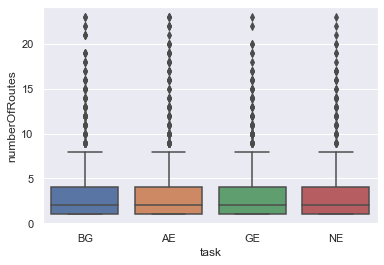
\includegraphics{contents/06_model_evaluation/res/Usage_Result_Overview.png}
    \caption{Anzahl der gefahrenen Routen für jede Studiengruppe}
\end{figure}

\begin{table}
    \begin{center}
        \begin{tabular}{|c|c|c|c|}
            \hline
            \textbf{Studiengruppe}  & \textbf{Mittelwert} [N] & \textbf{Standardabweichung} [N] \\ \hline
            Gruppe 1                & 3.2672 & 3.2958 \\ \hline
            Gruppe 2                & 3.2256 & 3.1961 \\ \hline
            Gruppe 3                & 4.6630 & 4.7043 \\ \hline
            Gruppe 4                & 4.5391 & 4.1509 \\ \hline
        \end{tabular}
    \end{center}
    \caption{Übersicht der Ergebnisse der gefahrenen Routen der Nutzer}
    \label{tab:study_offroute_results_2}
\end{table}

Zur Prüfung der Signifikanz wird wieder der Kruskal-Wallis-Test eingesetzt, da auch die Daten der Anzahl der gefahrenen Routen pro Studienteilnehmer nicht normalverteilt sind (Shapiro-Wilk: $ p = 0.0000 < 0.05 $). Mit $ p = 1.146748e-16 $ kann davon ausgegangen werden, dass ein Haupteffekt vorliegt.

Für die Prüfung zwischen welchen Studiengruppen ein signifikanter Unterschied vorliegt, wird auch hier der Dunn-Test verwendnet. Die Prüfung ergibt, dass jeweils ein signifikanter Effekt zwischen den Gruppen 3 und 4 gegenüber den Gruppen 1 und 2 vorliegt. Folglich kann abgeleitet werden, dass die Nutzer NUNAV häufiger verwenden, wenn sie die Erklärungen während der Navigation erhalten unabhängig davon, ob diese kombiniert mit den Erklärungen vor der Navigation erfolgen.

Die Hypothesen 4.1 und 4.2 müssen abgelehnt werden, da weder alle Erklärungstypen zu einer signifikant häufigeren Nutzung von NUNAV führen, noch das Geben von beiden vorgestellten Typen von Erklärungen zu einer erhöhten Nutzung pro Studienteilnehmer führt im Vergleich zur Präsentation von nur einem der integrierten Erklärungstypen.

\subsubsection{Bedarf für die gegebenen Erklärungen}

Die statischen Erklärungen (siehe \autoref{sec:user_count_definition} und \autoref{sec:route_explanation_definition}), welche die Einflüsse auf den Routing-Algorithmus von NUNAV sowie das kollaborative Routing erklären, sind interaktiv. Somit kann evaluiert werden, wie viele Studienteilnehmer wie häufig diese angefordert haben. Außerdem kann gemessen werden, wie lange sie die Erklärungen betrachtet haben.

Die drei verschiedenen Erklärungen, die die Nutzer aufrufen können, sind in \autoref{sec:user_count_definition} und \autoref{sec:route_explanation_definition} beschrieben. Die Studiengruppen (Gruppe 2 und 4), denen diese angezeigt wurden enthalten insgesamt 1 766 Teilnehmer.

Im Folgenden wird die Erklärung zum Routing-Algorithmus \textit{Erklärung 1}, die kurze Erklärung zum kollaborativen Routing als \textit{Erklärung 2} und die dazugehörige weitere Erklärung als \textit{Erklärung 3} genannt.

Als gelesen bzw. zumindest entschieden, ob die Erklärung benötigt wird gilt diese, wenn ein Nutzer länger als 1,5 Sekunden in dem Dialog verbracht hat \cite{BAHR2011776}. \autoref{fig:explanation_results_clicked} zeigt wie häufig die Nutzer eine Erklärung angefordert haben und diese auch zumindest zum Teil gelesen haben. \autoref{tab:explanation_results_clicked} zeigt die Bewertung als \glqq Hilfreich\grqq{} oder \glqq Nicht hilfreich\grqq{} durch die Nutzer. Allerdings sind die Hilfe-Artikel auch über andere Wege erreichbar, wodurch Bewertungen nicht nur von Nutzern kommen, die über die NUNAV-App dort hingeleitet wurden.

\begin{figure}
    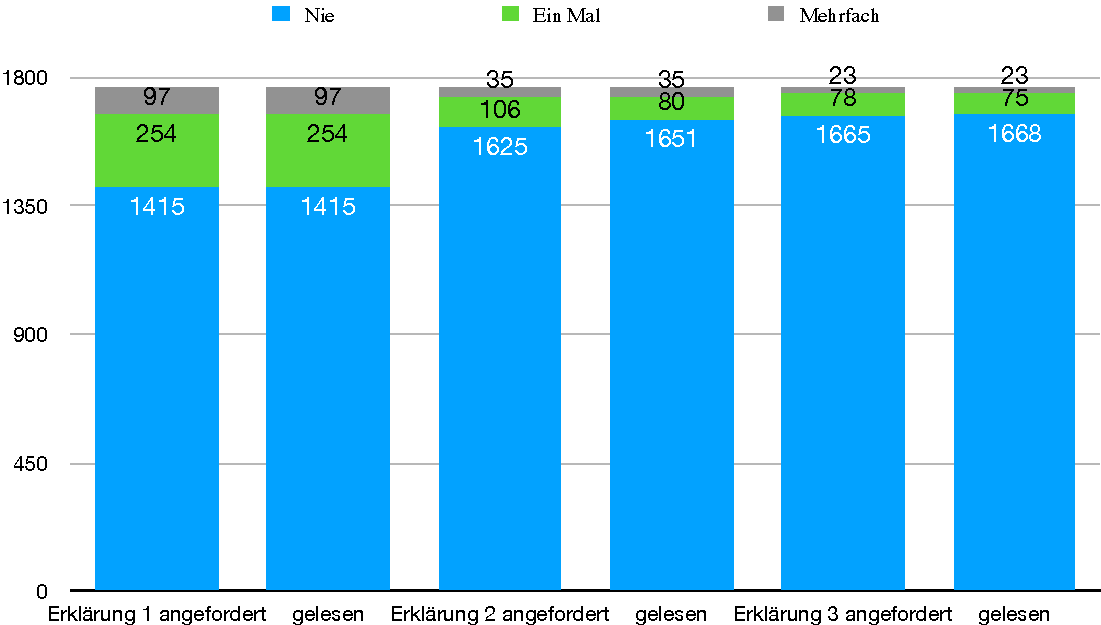
\includegraphics[width=\linewidth]{contents/06_model_evaluation/res/explanation_results_clicked.pdf}
    \caption{Anzahl der Klicks bzw. gelesenen Erklärungen}
    \label{fig:explanation_results_clicked}
\end{figure}

\begin{figure}
    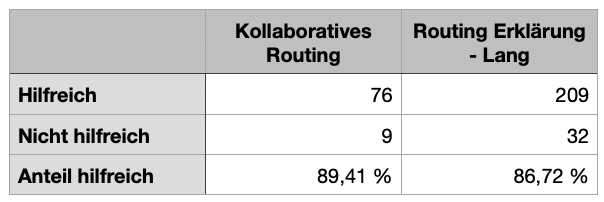
\includegraphics[width=\linewidth]{contents/06_model_evaluation/res/explanation_results_clicked_support.png}
    \caption{Bewertung der langen Erklärungen (Support-Artikel)}
    \label{tab:explanation_results_clicked}
\end{figure}

\subsubsection{Zusammenfassung}

% \begin{figure}
%     \text{Evaluation des Erklärungsbedarfs} \\
%     \subfloat[Anzahl der Teilnehmer, die Erklärung 1 angefordert haben]
%     {\includegraphics[width=.3\linewidth]{contents/06_model_evaluation/res/evaluation_explanation_1_clicks.pdf}}
%     \hspace{5mm}
%     \subfloat[Anzahl der Teilnehmer, die Erklärung 2 angefordert haben]
%     {\includegraphics[width=.3\linewidth]{contents/06_model_evaluation/res/evaluation_explanation_1_clicks.pdf}}
%     \hspace{5mm}
%     \subfloat[Anzahl der Teilnehmer, die Erklärung 2 angefordert haben]
%     {\includegraphics[width=.3\linewidth]{contents/06_model_evaluation/res/evaluation_explanation_1_clicks.pdf}} \\
%     \subfloat[Berechnete und reale Koordinaten]
%     {\includegraphics[width=.47\linewidth]{gfx/MagnetEvaluation/alg1-n48/grafic3.pdf}}
%     \hspace{5mm}
%     \subfloat[Relativer Rechenfehler]
%     {\includegraphics[width=.47\linewidth]{gfx/MagnetEvaluation/alg1-n48/grafic4.pdf}}
%     \caption[Evaluation der Positionsbestimmung mithilfe des Coulombschen Gesetzes]{Evaluation der Positionsbestimmung mithilfe des Coulombschen Gesetzes bei Verwendung eines Magneten mit Magnetisierungsgrad N48, 8 mm Durchmesser und 20 mm Länge}
%     \label{fig:evaluation_explanations_clicks}
% \end{figure}

Keinen Zusammenhang zwischen den Erklärungen und einer schlechteren / späteren ATA

\subsubsection{Qualitativ}
\label{sec:study_results_qualitativ}